\documentclass[a4paper, 11pt]{article}
\usepackage{geometry}
\usepackage{indentfirst}
\usepackage{setspace}
\usepackage{amsmath}
\usepackage{amssymb}
\usepackage{graphicx}
\usepackage{wrapfig}
\usepackage{caption}
\usepackage{indentfirst}
\setlength{\parindent}{20pt}
\usepackage{amssymb}
\usepackage{float}
\usepackage{subcaption}

\graphicspath{ {./images/} }
\geometry{left=2.5cm, right=2.5cm, top=2.5cm, bottom=2.5cm}

\begin{document}	
	\title{Lab Exercise}
	\author{{\small Alexandre Rodrigues (2039952)}}
	\date{\today}
	\maketitle
	
	\section{Introduction}
		The objective of this exercise is to find the minimum time needed to drill all the holes in a electric panel.
		For part 1, I used the model described in the exercise text.
		For part 2, I used the Tabu Search with Aspiration Criteria, made some changes and added a heuristic initial solution procedure.
		
		
	\section{Technical Approach}
	
		\subsection{Cplex model}
			\textbf{Sets:}
			\begin{itemize}
				\item $ N = $ graph nodes, representing the holes;
				\item $ A = arcs (i,j), \forall i,j \in N $, representing the trajectory covered by the drill to move from hole $ i $ to hole $ j $.
			\end{itemize}
		
			\textbf{Parameters:}
			\begin{itemize}
				\item $ c_{ij} = $ time taken  by the drill to move from $ i to j,\forall (i,j) \in A $ ;
				\item $ 0 = $ arbitrarily selected starting node, $ 0 \in N $.
			\end{itemize}
		
			\textbf{Decision variables:}
			\begin{itemize}
				\item $ x_{ij} = $ amount of the flow shipped from $ i to j,\forall (i,j) \in A $ ;
				\item $ y_{ij} = 1 $ if arc $ (i,j) $ ships some flow, $ 0 $ otherwise, $\forall (i,j) \in A $ ;
			\end{itemize}
		
		
				
			The improved formulation in the exercise text is the following:
			\begin{align}
				min &\sum_{i,j:(i,j)\in A} c_{ij} y_{ij}\\
				s.t &\sum_{i:(i,k)\in A} x_{ik} - \sum_{j:(k,j),j\ne 0} x_{kj} &= 1 \qquad\qquad\qquad &\forall k \in N \backslash 0 \\
				&\sum_{j:(i,j)\in A} 	&= 1 \qquad \qquad \qquad 				&\forall i \in N \\
				&\sum_{i:(i,j)\in A} 	&= 1 \qquad \qquad \qquad 				&\forall j \in N \\
				&x_{ij}  				&\le (|N|-1) y_{ij} \quad 	&\forall (i,j) \in A, j\ne 0 \\
				&x_{ij}  \in R_+ 		&   						&\forall (i,j) \in A, j\ne 0 \\
				&y_{ij}  \in \{0,1\} 	&  							&\forall (i,j) \in A \\
			\end{align}
				
		
		
		\subsection{Instancing}
			Class 1 - Random
				Randomly selected n positions of the n x n map.
				Then compute the cost matrix.
				
				Implementation:
				1. Compute all possible positions (3x3 example)
					(0,0) (0,1) (0,2) 
					(1,0) (1,1) (1,2)
					(2,0) (2,1) (2,2)
				2. Randomly shuffle them
				3. Select the first n positions from the set.
				
			
			Class 2 - Domain specific random
				Same as before but for a n-1 x n-1 map.
				Limited to {1,2,$\ldots$,N-2} instead of {0,2,$\ldots$,N-1}.
				This because there are basically no electric panels with holes near the border.
				
			Class 3 - Handmade instances for n = 10	
				I created the following 6 instances from what seemed more realistic.
				I then created the positions files and a function to compute the cost matrix.
				
				\begin{figure}[H]
					\centering
					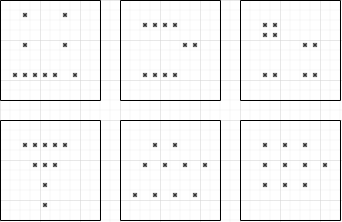
\includegraphics[width=.99\linewidth]{class3.png}  
					\caption{Instances of class 3}
					\label{fig:figsClass3}
				\end{figure}
			
			
			
			
			
			
		\subsection{part2}

			I started from the TSAC implementation from the Labs.
			I implemented the same initialization methods from part1.
			1 to randomly select holes positons (either class1 or class1 DS).
			1 to compute the costs matrix from these positions.
			1 to read from the dists10 intansces as they use positions
			1 to better seed the random methods with a mix() function.
			
			Additional Heuristic initialization:
				Iterate the cost matrix and find the minimum value in each row, excluding the already visited nodes.
						
	
	\section{Results}
		I tested class 3 only for n=10 with 6 instances, 5 runs each.
		The cost matrix was computed from the hole positions (random or not) using Manhattan distance.
		The class 2 instances are random but slightly domain specific.
		In this case I simply removed the possibility to have holes in the borders of the board.
		
		Class 1 is fully random:
		board as size = N
		so $ x \in {0,N-1}$
		hole of size 1
		
		Both class 1 and 2 were tested using 30 random instances for $ 10 \le n \le 70 $.
		Due to the considerable time I reduced it to 10 instances for $ 80 \le n \le 100 $.
		Each instance was run 5 times to get the average computational time.
		
		The time to drill a hole is constant so we can disregard it.
		The total cost would be $ cost_{real}  = cost_{exp} + cN, c\in \mathbb{R}$.
		
		\begin{table}[H]
			\centering
			\begin{tabular}{c|c|c|c}
				\textbf{Comparison}& \textbf{exact} & \textbf{TSAC1}  			& \textbf{TSAC2}  \\ \hline
				Time			& $ 0.1165 s $ 		& $ 4.05 \times 10^{-5} s $ 	& $ 1.06 \times 10^{-5} s $ \\ \hline
				InitialSol		& N/A		 		& $ 47.4 $ 						& $ 24.0 $ \\ \hline 
				FinalValue		& $ 22.33 $	 		& $ 22.5 $ 						& $ 22.33 $ \\  
			\end{tabular}
			\caption{Comparison for class3}
			\label{table:times3}
		\end{table}
		TSAC is clearly faster to converge
		Using an heuristic initial solution improves convergence time and final solutions found.
		On can also see that our initial heuristic solution is half of the random initial solytoons.
		This will be even more noticeable for larger n, however the time differences will become desprezabel.
		
	
		
		\begin{table}[H]
			\centering
			\begin{tabular}{c|c|c}
				\textbf{$ n $} 	& \textbf{class1} 	& \textbf{class2}  \\ \hline
				$ 10  $			& $ 0.1199 s $ 		& $ 0.1285 s $ \\ \hline
				$ 20  $			& $ 0.430 s $ 		& $ 0.461 s $ \\ \hline
				$ 30  $			& $ 1.575 s $	 	& $ 1.397 s $ \\ \hline
				$ 40  $			& $ 6.603 s $ 		& $ 6.570 s $ \\ \hline
				$ 50  $			& $ 14.04 s $ 		& $ 14.55 s $ \\ \hline
				$ 60 $			& $ 28.80 s $ 		& $ 28.14 s $ \\ \hline
				$ 70 $			& $ 46.66s $	 	& $ 53.88 s $ \\ \hline
				$ 80 $			& $ 90.96 s $ 		& $ 86.53 s $ \\ \hline
				$ 90 $			& $ 215.1 s $	 	& $ 207.97 s $ \\ \hline
				$ 100 $			& $ 458.5 s $ 		& $ 312.64 s $ \\ 
			\end{tabular}
			\caption{Average Time for Exact}
			\label{table:times}
		\end{table}
		There are no notcieable differences reagrding convergence time between the classes.
		
		
		For part2 the TSAC method found a good enough solution in a maximum of 0.0082 seconds for n=100.
		Ther were no significant differences between the classes and initializatuion methods used.
	
		
		Assuming a max time as 20 seconds.... we can solve for up to 50 nodes.
		
		
	\begin{table}[H]
		\centering
		\begin{tabular}{c|c|c|c|c}
			\textbf{$ n $} 	& \textbf{class1} & \textbf{class1 init2}  & \textbf{class2} & \textbf{class2 init2}  \\ \hline
			$ 10  $			& $1.54\times10^{-5}$ & $9.35\times10^{-6}$& $1.97\times10^{-5}$ & $1.04\times10^{-5}$ \\ \hline
			$ 20  $			& $9.11\times10^{-5}$ & $1.40\times10^{-4}$& $1.00\times10^{-4}$ & $1.21\times10^{-4}$ \\ \hline
			$ 30  $			& $2.33\times10^{-4}$ & $2.54\times10^{-4}$& $2.31\times10^{-4}$ & $3.47\times10^{-4}$ \\ \hline
			$ 40  $			& $3.49\times10^{-4}$ & $7.53\times10^{-4}$& $3.42\times10^{-4}$ & $7.22\times10^{-4}$\\ \hline
			$ 50  $			& $7.97\times10^{-4}$ & $6.74\times10^{-4}$& $6.68\times10^{-4}$ & $9.80\times10^{-4}$ \\ \hline
			$ 60  $			& $1.13\times10^{-3}$ & $2.18\times10^{-3}$& $1.70\times10^{-3}$ & $2.05\times10^{-3}$ \\ \hline
			$ 70 $			& $1.91\times10^{-3}$ & $2.54\times10^{-3}$& $3.16\times10^{-3}$ & $3.11\times10^{-3}$\\ \hline
			$ 80 $			& $2.56\times10^{-3}$ & $3.96\times10^{-3}$& $2.97\times10^{-3}$ & $3.07\times10^{-3}$\\ \hline
			$ 90 $			& $4.98\times10^{-3}$ & $5.93\times10^{-3}$& $3.87\times10^{-3}$ & $5.73\times10^{-3}$\\ \hline
			$ 100 $			& $5.83\times10^{-3}$ & $8.20\times10^{-3}$& $5.14\times10^{-3}$ & $8.66\times10^{-3}$\\
		\end{tabular}
		\caption{Average Time for TSAC}
		\label{table:times2}
	\end{table}

	All this computational times are below 1 second, so very easily solvable.
	As an extra test, for n=1000, times are around 5 seconds.
	The following tables show the final solution values obtained



	\begin{table}[H]
		\centering
		\begin{tabular}{c|c|c|c|c|c}
			\textbf{$ n $} 	& \textbf{exact} & \textbf{initial1}   & \textbf{final1}& \textbf{initial2} & \textbf{final2} 	\\ \hline
			$ 10  $			& $ 34.067 $ 	& $ 66.067 $ 			& $ 34.067 $  	& $ 38.067 $ 		& $ 34.067 $		\\ \hline
			$ 20  $			& $ 94.33 $ 	& $ 258.2 $ 			& $ 95.067 $  	& $ 110.8 $ 		& $ 94.933 $		\\ \hline
			$ 30  $			& $ 167.067 $ 	& $ 606.53 $ 			& $ 170.2 $  	& $ 202.6 $ 		& $ 169.6 $ \\ \hline
			$ 40  $			& $ 257.4 $ 	& $ 1076.87 $ 			& $ 266.3 $  	& $ 310.8 $ 		& $ 263.93 $ \\ \hline
			$ 50  $			& $ 356.6 $ 	& $ 1630.47 $ 			& $ 366.8 $  	& $ 428.067 $ 		& $ 366.467 $ \\ \hline
			$ 60  $			& $ 461.93 $ 	& $ 2418.6 $ 			& $ 482.73 $  	& $ 570.4 $ 		& $ 479.267 $ \\ \hline
			$ 70 $			& $ 578.93 $ 	& $ 3264.13 $ 			& $ 607.93 $  	& $ 732.73 $ 		& $ 599.6 $ \\ \hline
			$ 80 $			& $ 703.4 $ 	& $ 4343.2 $ 			& $ 739.6 $  	& $ 869.6 $ 		& $ 724.2 $ \\ \hline
			$ 90 $			& $  $ 		& $ 5476.8 $ 			& $ 888.2 $  	& $ 1052.2 $ 		& $ 869 $ \\ \hline
			$ 100 $			& $  $ 		& $ 6670.2 $ 			& $ 1042 $  	& $ 1228.2 $ 		& $ 1013.4 $ \\
		\end{tabular}
		\caption{Solutions for class1}
		\label{table:sols}
	\end{table}
	
	\begin{table}[H]
		\centering
		\begin{tabular}{c|c|c|c|c|c}
			\textbf{$ n $} 	& \textbf{exact} & \textbf{initial1}   & \textbf{final1}& \textbf{initial2} & \textbf{final2} 	\\ \hline
			$ 10  $			& $ 28.533 $ 	& $ 52.333 $ 			& $ 28.533 $  	& $ 32 $ 			& $ 28.533 $		\\ \hline
			$ 20  $			& $ 84.467 $ 		& $ 233.13 $ 			& $ 84.733 $  	& $ 98 $ 			& $ 84.6$		\\ \hline
			$ 30  $			& $ 160.933 $ 	& $ 562.73 $ 			& $ 164.4 $  	& $ 197.53 $ 		& $ 163.067 $ \\ \hline
			$ 40  $			& $ 243.4 $ 	& $ 1040.4 $ 			& $ 252.53 $  	& $ 289.33 $ 		& $ 248.8 $ \\ \hline
			$ 50  $			& $ 339.73 $ 		& $ 1583.53 $ 			& $ 350.2 $  	& $ 412.4 $ 		& $ 346.53 $ \\ \hline
			$ 60  $			& $ 445 $ 	& $ 2356.67 $ 			& $ 466.2 $  	& $ 527.93 $ 		& $ 458.267 $ \\ \hline
			$ 70 $			& $ 560.13 $ 	& $ 3203.8 $ 			& $ 593.6 $  	& $ 898.867 $ 		& $ 582.4 $ \\ \hline
			$ 80 $			& $ 687.6 $ 	& $ 4163.4 $ 			& $ 730 $  		& $ 859.8 $ 		& $ 711.2 $ \\ \hline
			$ 90 $			& $  $ 		& $ 5358.4 $ 			& $ 845.4 $  	& $ 1016 $ 			& $ 845 $ \\ \hline
			$ 100 $			& $  $ 	& $ 6665 $ 				& $ 1022 $  	& $ 1172.2 $ 		& $ 988$ \\
		\end{tabular}
		\caption{Solutions for class2}
		\label{table:sols2}
	\end{table}

	The initialization using the min each row heuristic is clearly a better approximation to the optimal solution.
	
	We can although notice a tendency to worse solutions when we increase n.
	
	
	
	
	
	NOTE: After most testing there as a clear slowdown due to someone running an intensive program in the Math department server I was using.
	There were some bug fixes after this but only the solution values were saved and used in this report. 
	Computational time should ideally be approximately the ones showed here.
	
	\section{Conclusions}
	
	
\end{document}



